\chapter{Introducción a aplicaciones}
Esta clase tiene como objetivo aplicar los conceptos estudiados durante el curso en distintas aplicaciones utilizando imágenes de distintos satélites.

\section{Detección de espejos de agua}

Para la detección se espejos de agua, utilizando imágenes \emph{Sentinel 1}, durante octubre de 2017 en la zona de Chascomús, provincia de Buenos Aires, Argentina.

% Imagen antes
% S1B_IW_GRDH_1SDV_20171007T090618_20171007T090643_007721_00DA33_E6D1

% Subset
% N = -35.632
% W = -57.395
% S = -35.933
% E = -58.569

\subsection{Actividades}

\begin{que}
    Descargue la imagen del 7 de octubre del 2017
    \begin{center}\path{ S1B_IW_GRDH_1SDV_20171007T090618_20171007T090643_007721_00DA33_E6D1}\end{center} del \href{https://vertex.daac.asf.alaska.edu/}{Alaska Satellite Facility}. Utilice la búsqueda por \emph{Granule} en lugar de la \emph{Geospatial}.
\end{que}

\begin{que}
    Con la herramienta \menu{Raster>Subset} (Figura \ref{fig:coordenadas})
    \begin{figure}[h!]
        \centering
        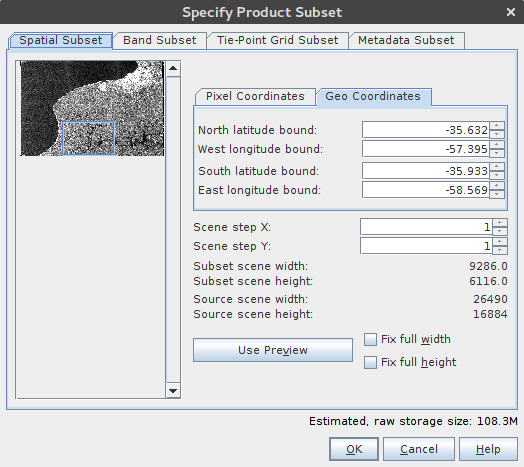
\includegraphics[scale=0.35]{fig:coordenadas.png}
        \caption{Subset espacial de una imagen en SNAP. Se reliza en este caso utilizando las coordenadas geográficas.}
        \label{fig:coordenadas}
    \end{figure}
    haga un recorte entre las coordenadas geográficas
    \begin{itemize}
        \item Latitud norte: -35.632
        \item Longitud oeste: -57.395
        \item Latitud sur: -35.933
        \item Longitud este: -58.569
    \end{itemize}
\end{que}

\begin{que}
    Procese la imagen como se realizó en la clase 3. Calíbrela para obtener el coeficiente de backscatter, aplique los filtros correspondientes y proyectela en terreno utilizando un DEM. Exporte la vista obtenida en dB.
\end{que}

\begin{que}
    En la imagen, identifique cuerpos de agua, vegetación y ciudades. Mida su coeficiente de retrodispersión en las bandas VV y VH. Seleccione que polarización separa mejor las zonas con y sin agua.
\end{que}

\begin{que}
    Utilizando la herramienta \menu{Analysis>Histogram} calcule el histograma de la imagen e identifique un valor por debajo del cual, el coeficiente de retrodispersión corresponde a agua.
\end{que}

\begin{que}
    Obtenga un mapa de zonas anegadas. Utilice la herramienta \menu{Band math...} (Apéndice \ref{ap:HA}) con click derecho sobre el nombre de la imagen e ingrese la formula
    \begin{center}
        \path{BANDA < T}
    \end{center}
    donde T es el valor obtenido en el punto anterior. Haga click derecho sobre la nueva banda y en propiedades ingrese 0 en \emph{No-Data Value}.
\end{que}

\begin{que}
    Exporte el mapa como KMZ (Apéndice \ref{ap:GE}).
\end{que}


\section{Detección derrames de aceite}

Para la detección se derramos de aceite y petroleo, utilizando imágenes \emph{Sentinel 1}.

% Imagen antes
% S1A_IW_GRDH_1SDV_20170311T021505_20170311T021528_015638_019B8B_9D85
% S1A_IW_GRDH_1SDV_20170308T142434_20170308T142459_015602_019A78_F8CB
%

% Subset
% N = 25.313
% W = 53.930
% S = 26.089
% E = 54.933

\subsection{Actividades}

\begin{que}
    Descargue la imagen del 7 de octubre del 2017
    \begin{center}\path{ S1A_IW_GRDH_1SDV_20170102T063506_20170102T063531_014649_017D2D_D901}\end{center} del \href{https://vertex.daac.asf.alaska.edu/}{Alaska Satellite Facility}. Utilice la búsqueda por \emph{Granule} en lugar de la \emph{Geospatial}.
\end{que}

\begin{que}
    Con la herramienta \menu{Raster>Subset} (Apéndice \ref{ap:HA}) haga un recorte entre las coordenadas geográficas
    \begin{itemize}
        \item Latitud norte:
        \item Longitud oeste:
        \item Latitud sur:
        \item Longitud este:
    \end{itemize}

\end{que}

\begin{que}
    Procese la imagen como se realizó en la clase 3. Calíbrela para obtener el coeficiente de backscatter, aplique los filtros correspondientes y proyectela en terreno utilizando un DEM. Exporte la vista obtenida en dB.
\end{que}

\begin{que}
    En la imagen, identifique zonas con agua y aceite. Estas últimas se observarán más oscuras. Mida su coeficiente de retrodispersión en las bandas VV y VH. Seleccione que polarización separa mejor las zonas con y sin aceite.
\end{que}


\begin{que}
    Utilizando la herramienta \menu{Analysis>Histogram} calcule el histograma de la imagen e identifique un valor por debajo del cual, el coeficiente de retrodispersión corresponde a agua.
\end{que}

\begin{que}
  Obtenga un mapa de zonas anegadas. Utilice la herramienta \menu{Band math...} (Apéndice \ref{ap:HA}) con click derecho sobre el nombre de la imagen e ingrese la formula
  \begin{center}
      \path{BANDA < T}
  \end{center}
  donde T es el valor obtenido en el punto anterior.
\end{que}

\begin{que}
    Exporte el mapa como KMZ (Apéndice \ref{ap:GE}).
\end{que}


\section{Deforestación en Salta}

% Imagen antes
% S1A_IW_GRDH_1SSV_20141122T224900_20141122T224925_003400_003F6A_A171
% S1B_IW_GRDH_1SDV_20171124T224831_20171124T224859_008429_00EEE9_992C
% Subset
% N = -24.345
% W = -63.925
% S = -23.724
% E = -63.291

\subsection{Actividades}

\begin{que}
    Descargue las imagenes del 22 y 24 de noviembre de los años 2014 y 2017.
    \begin{center}\path{ S1A_IW_GRDH_1SSV_20141122T224900_20141122T224925_003400_003F6A_A171}\end{center}
      \begin{center}\path{ S1B_IW_GRDH_1SDV_20171124T224831_20171124T224859_008429_00EEE9_992C}\end{center}
      del \href{https://vertex.daac.asf.alaska.edu/}{Alaska Satellite Facility}. Utilice la búsqueda por \emph{Granule} en lugar de la \emph{Geospatial}.
\end{que}

\begin{que}
    Con la herramienta \menu{Raster>Subset} (Apéndice \ref{ap:HA}) haga un recorte entre las coordenadas geográficas
    \begin{itemize}
        \item Latitud norte: -24.345
        \item Longitud oeste: -63.925
        \item Latitud sur: -23.724
        \item Longitud este: -63.291
    \end{itemize}
\end{que}

\begin{que}
    Procese la imagen para la banda VV como se realizó en la clase 3. Calíbrela para obtener el coeficiente de backscatter, aplique los filtros correspondientes y proyectela en terreno utilizando un DEM. Exporte la vista obtenida en dB para cada imagen.
\end{que}

\begin{que}
    En la imagen, identifique cuerpos de agua, vegetación y suelos sin cobertura. Mida su coeficiente de retrodispersión en las bandas VV.
\end{que}

\begin{que}
    Obtenga un mapa de cambio. Utilice la herramienta \menu{Band math...} (Apéndice \ref{ap:HA}) haga la diferencia entre las bandas de las imágenes
    \begin{center}
        \path{IMAGEN2017.Sigma0_VV - IMAGEN2014.Sigma0_VV}
    \end{center}
    Puede utilizar la opción \menu{Edit expression...} para ingresar la formula.
\end{que}


\begin{que}
    Utilizando la herraamienta \menu{Pixel info} obtenga un valor de umbral por debajo del cual considera que hubo deforestación
\end{que}

\begin{que}
    Obtenga un mapa de zonas deforestadas. Utilice la herramienta \menu{Band math...} (Apéndice \ref{ap:HA}) con click derecho sobre el nombre de la imagen e ingrese la formula
    \begin{center}
        \path{BANDA < T}
    \end{center}
    donde T es el valor obtenido en el punto anterior. Haga click derecho sobre la nueva banda y en propiedades ingrese 0 en \emph{No-Data Value}.
\end{que}

\begin{que}
    Exporte el mapa como KMZ (Apéndice \ref{ap:GE}).
\end{que}


\section{Expansión urbana}

% Imagen antes
% S1A_IW_GRDH_1SDV_20171204T155928_20171204T155953_019555_021343_887D
% S1A_IW_GRDH_1SDV_20141009T155904_20141009T155929_002755_003184_0439
% Subset
% N = 40.597
% W = 28.450
% S = 41.268
% E = 29.534
